\section{Experiments}
\label{sec:exp}

We evaluate \methodname\ on large-scale enzyme screening, bidirectional
enzyme--reaction retrieval, and a literature-derived enzyme panel. The
experiments address three questions: whether the model improves early
enzyme recovery, whether its representations transfer across retrieval
settings, and which training and inference choices account for the observed
performance. Following FGW-CLIP \citep{zhou2026fgwclip}, we use EnzymeMap for
screening and ReactZyme for bidirectional retrieval. Case1 assesses
retrospective catalyst prioritization outside these benchmark candidate pools.

\paragraph{Implementation.}
We fit the same architecture and hyperparameter recipe separately to each
benchmark training partition. The F3 retrieval layers are freshly initialized;
the pretrained feature extractors remain frozen. Phase 1 uses anchor-balanced
decoupled multi-positive learning with inverse temperature $\beta=5$, batch
size 512, and AdamW with learning rate $10^{-4}$ and weight decay $10^{-2}$
for 10 epochs. Phase 2 freezes F3 and trains the residual heads for 100
full-graph updates using uniform-positive cross-entropy, temperature 0.2,
and identity-penalty weight 10. Its learning rate is $10^{-4}$ and weight
decay is $10^{-3}$. At inference, the training-reaction dictionary weight is
$\alpha=0.40$, protein fusion multiplier is $\nu=3$, and residual multiplier
is $c=0.5$. We use neither ensembles nor hubness correction.
The proposed method uses no added biological-label loss; this supervision
is evaluated only as an ablation in Section~\ref{sec:exp-ablation}.
Primary results use seed 42.
Downstream associations are matched across local comparisons, while pretrained
representations and auxiliary annotations remain method-specific.

\subsection{Enzyme screening on EnzymeMap}
\label{sec:exp-screening}

\paragraph{Datasets.}
We adopt the processed EnzymeMap dataset and reaction-rule split distributed
with CLIPZyme \citep{heid2023enzymemap,mikhael2024clipzyme}. The dataset
contains 46,356 associations, 16,776 reactions, 12,749 enzymes, 2,841 EC
identifiers, and 394 reaction rules. The released rule-based 80/10/10 split
contains 34,427 training, 7,287 validation, and 4,642 test associations. The
screening library combines EnzymeMap, BRENDA 2022\_2, and UniProt 2022\_01,
and contains 261,907 candidate identifiers with sequences of at most 650
residues. We retain the released reactant/product roles and candidate library.

Following the released CLIPZyme notebook, the 4,642 test associations yield
1,551 distinct reaction strings; removing 30 that also occur in training
leaves 1,521 screening queries. Positives are the corresponding protein
identifiers in the raw EnzymeMap records intersected with the screening
library, giving 4,544 positive query--candidate labels. We evaluate both the
\emph{full library} and a \emph{training-ID-excluded library}, following the
additional FGW-CLIP analysis. The latter contains 252,113 candidates and
1,337 queries with remaining positives. Identifier exclusion does not enforce
sequence- or homology-disjointness.

\paragraph{Baselines and metrics.}
We compare with the reported CLIPZyme variants and FGW-CLIP, and evaluate
the released CLIPZyme checkpoint locally using the same candidate axes,
query eligibility, and positive labels as our model. This checkpoint was
trained on the corresponding EnzymeMap partition. FGW-CLIP is a published
reference rather than a local reproduction, as no verified executable
release was available for these experiments. We report query-averaged
BEDROC$_{85}$, BEDROC$_{20}$, EF5, and EF10; higher is better. BEDROC is shown
as a percentage in Table~\ref{tab:exp-screening}. For $n$ positives among $N$ candidates, enrichment
at fraction $f$ is $\mathrm{EF}_f=\sum_{j=1}^{\lfloor fN\rfloor}y_{(j)}/(fn)$,
where $y_{(j)}$ is the ranked positive label. We preserve the released
notebook's zero-based BEDROC ranks and sorting convention. MRR is not a
screening endpoint.

\begin{table}[t]
\centering\small
\caption{EnzymeMap screening. BEDROC values are percentages; EF values are
fold enrichments. $\dagger$ denotes published results from FGW-CLIP;
CLIPZyme (released) is evaluated locally. The full and excluded libraries
contain 261,907 and 252,113 candidates, respectively. Bold marks the best
locally evaluated result in each column.}
\label{tab:exp-screening}
% Generated from bundled frozen evidence; stages uses stage_comparison.json.
\begingroup\setlength{\tabcolsep}{2.8pt}
\begin{tabular}{@{}lrrrrrrrr@{}}
\toprule
Method & \multicolumn{4}{c}{Full library} & \multicolumn{4}{c}{Training-ID-excluded} \\
\cmidrule(lr){2-5}\cmidrule(lr){6-9}
 & B$_{85}$ & B$_{20}$ & EF5 & EF10 & B$_{85}$ & B$_{20}$ & EF5 & EF10 \\
\midrule
CLIPZyme (ESM)$^\dagger$ & 36.91 & 53.04 & 11.93 & 6.84 & -- & -- & -- & -- \\
CLIPZyme (CGR)$^\dagger$ & 38.91 & 57.58 & 13.16 & 7.73 & -- & -- & -- & -- \\
CLIPZyme$^\dagger$ & 44.69 & 62.98 & 14.09 & 8.06 & 39.13 & 58.86 & 13.40 & 7.81 \\
FGW-CLIP$^\dagger$ & 48.66 & 66.69 & 14.91 & 8.18 & 45.14 & 61.43 & 13.57 & 7.61 \\
\midrule
CLIPZyme (released) & 44.69 & 62.98 & 14.09 & 8.06 & 39.13 & 58.86 & 13.40 & 7.81 \\
\methodname & \textbf{57.23} & \textbf{75.54} & \textbf{16.86} & \textbf{8.96} & \textbf{52.87} & \textbf{72.64} & \textbf{16.42} & \textbf{8.79} \\
\bottomrule
\end{tabular}
\endgroup

\end{table}

\paragraph{Results.}
Table~\ref{tab:exp-screening} shows that \methodname\ improves all four
screening endpoints over the released CLIPZyme checkpoint and the reported
FGW-CLIP values in both libraries. Full-library BEDROC$_{85}$ reaches
57.23\%, compared with 44.69\% for released CLIPZyme and 48.66\% for
FGW-CLIP, gains of 12.54 and 8.57 percentage points. EF5 increases from
14.09 and 14.91 to 16.86. After excluding training identifiers,
BEDROC$_{85}$ remains 52.87\% and EF5 is 16.42. The improvement therefore
persists when training identifiers cannot be retrieved.

\subsection{Bidirectional retrieval on ReactZyme}
\label{sec:exp-reactzyme}

\paragraph{Datasets.}
ReactZyme associates SwissProt enzymes with Rhea reactions and provides
reaction-similarity, enzyme-similarity, and temporal splits
\citep{hua2024reactzyme}. The released resource comprises 178,463
associations, 178,327 enzymes, and 7,726 reaction identifiers. We preserve
the existing training, validation, and test partitions, with retained counts
in Table~\ref{tab:exp-data}. Each split contains 178,459 retained association
rows. The temporal split uses the released 31 December 2010 cutoff. All
local methods use the same complete test query and candidate catalogs in
each direction. ReactZyme supplies flattened reaction participants in this
materialization; its self-reaction encoding does not recover physical
reactant/product roles.

\begin{table}[t]
\centering\small
\caption{ReactZyme partitions used by every local method. Train/validation/test
columns count association rows; $|R_{\rm test}|$ and $|E_{\rm test}|$ are
the complete test catalogs, whose query/candidate roles swap by direction.}
\label{tab:exp-data}
% Generated from bundled frozen evidence; stages uses stage_comparison.json.
\begingroup\setlength{\tabcolsep}{2.8pt}
\begin{tabular}{@{}lrrrrr@{}}
\toprule
Split & Train & Val. & Test & $|R_{\rm test}|$ & $|E_{\rm test}|$ \\
\midrule
Reaction-Sim & 147,393 & 16,377 & 14,689 & 386 & 14,688 \\
Enzyme-Sim & 152,748 & 16,972 & 8,739 & 1,573 & 8,734 \\
Time & 149,554 & 16,618 & 12,287 & 2,634 & 12,277 \\
\bottomrule
\end{tabular}
\endgroup

\end{table}

\paragraph{Baselines.}
We report two comparison groups. Published references include FGW-CLIP's
EC Mode/Max variants and TIGER's main ESM2Text/ProtT3 variants
\citep{zhou2026fgwclip,zhang2026tiger}. Local comparisons retrain the released
MLP, contrastive MLP, Transformer, and Bi-RNN families on the same downstream
partitions as V4. For a compact controlled presentation, we show their
ESM2/MAT-2D configuration throughout, together with a corrected contrastive-label
sensitivity, an EnzGFM backbone control, and original Horizyn
\citep{rocks2026horizyn}. This feature pair is fixed across families rather
than selected by test performance. The public-model campaign covers 126
completed configurations; its complete run inventory is retained separately.

The classifier baselines use four deterministic negative corruptions per
positive, excluding known positives, because the original negative files
are unavailable. They select checkpoints by validation BCE, with at most
200 epochs and patience 30. The corrected contrastive row resolves opposite
label conventions in the released BCE and contrastive branches. Horizyn
uses its original MLP towers, fingerprints, ProtT5 features, and MLNCE loss,
with a participant-set reaction adapter; it trains for at most 100 epochs
and selects by validation MRR. The EnzGFM row is a frozen-backbone control
with adapted preprocessing. These comparisons match downstream associations
but differ in inputs, objectives, and optimization budgets.

\paragraph{Metrics.}
For query $q$, let $P(q)$ denote its positive candidates and
$\mathrm{rank}_q(p)$ their one-based ranks. We use the benchmark
implementation's query-averaged all-positive reciprocal rank,
\begin{equation}
\mathrm{MRR}_{\rm all}=\frac{1}{|Q|}\sum_{q\in Q}
\frac{1}{|P(q)|}\sum_{p\in P(q)}\frac{1}{\mathrm{rank}_q(p)}.
\label{eq:exp-mrr}
\end{equation}
Local scores use FP32 ranking and stable candidate-index tie breaking.
First-positive MRR is a different quantity. Because published descriptions
such as FGW-CLIP's formula use the first positive, and predictions are
unavailable to reconcile the implementation, published values are kept
separate from the common-evaluator results.

\begin{table}[t]
\centering\small
\caption{ReactZyme retrieval. The upper group contains published MRR
($\dagger$); the lower group uses the shared all-positive evaluator in
Eq.~\ref{eq:exp-mrr}. Released-family rows use ESM2/MAT-2D; the EnzGFM
control uses MAT-2D. Training budgets and pretrained inputs differ. Bold
marks the best local value; display precision does not resolve very small
differences.}
\label{tab:exp-reactzyme}
% Generated from bundled frozen evidence; stages uses stage_comparison.json.
\begingroup\setlength{\tabcolsep}{2.8pt}
\begin{tabular}{@{}lrrrrrr@{}}
\toprule
Method & \multicolumn{2}{c}{Reaction-Sim} & \multicolumn{2}{c}{Enzyme-Sim} & \multicolumn{2}{c}{Time} \\
\cmidrule(lr){2-3}\cmidrule(lr){4-5}\cmidrule(lr){6-7}
 & R$\to$E & E$\to$R & R$\to$E & E$\to$R & R$\to$E & E$\to$R \\
\midrule
FGW-CLIP (EC Mode)$^\dagger$ & 0.3181 & 0.3722 & 0.5253 & 0.8683 & 0.3394 & 0.5222 \\
FGW-CLIP (EC Max)$^\dagger$ & 0.3113 & 0.3804 & 0.5300 & 0.8581 & 0.3392 & 0.5229 \\
TIGER (ESM2Text)$^\dagger$ & 0.3190 & 0.5180 & 0.5920 & 0.9560 & 0.3660 & 0.6900 \\
TIGER (ProtT3)$^\dagger$ & 0.3370 & 0.4720 & 0.5790 & 0.9400 & 0.3720 & 0.6830 \\
\midrule
MLP & 0.1057 & 0.2187 & 0.2155 & 0.7080 & 0.1046 & 0.2849 \\
Contrastive MLP & 0.0406 & 0.2398 & 0.1198 & 0.6667 & 0.0405 & 0.2550 \\
Transformer & 0.1220 & 0.2314 & 0.2163 & 0.7260 & 0.1419 & 0.3943 \\
Bi-RNN & 0.1510 & 0.2835 & 0.2736 & 0.7970 & 0.1274 & 0.3752 \\
Corrected contrastive & 0.0638 & 0.2431 & 0.1047 & 0.6316 & 0.0410 & 0.2412 \\
EnzGFM control & 0.1354 & 0.2965 & 0.2864 & 0.7989 & 0.1525 & 0.3867 \\
Horizyn (adapted) & \textbf{0.4318} & \textbf{0.5348} & \textbf{0.6997} & \textbf{0.9770} & \textbf{0.5982} & \textbf{0.8406} \\
\midrule
\methodname & 0.4004 & 0.5344 & 0.6662 & 0.9714 & 0.5383 & 0.7807 \\
\bottomrule
\end{tabular}
\endgroup

\end{table}

\paragraph{Results.}
\methodname\ achieves R$\to$E/E$\to$R MRR of 0.4004/0.5344 on Reaction-Sim,
0.6662/0.9714 on Enzyme-Sim, and 0.5383/0.7807 on Time
(Table~\ref{tab:exp-reactzyme}). These exceed the displayed main-method
literature values, subject to the metric distinction above. However,
original Horizyn exceeds \methodname\ in all six locally evaluated
cells. Its R$\to$E MRR is 0.4318 on Reaction-Sim and 0.5982 on Time,
compared with 0.4004 and 0.5383 for V4.
Thus V4's strong screening performance does not imply dominance in
bidirectional retrieval. The larger Horizyn training budget also prevents
isolating architecture as the cause of this ordering.

\subsection{Ablation studies}
\label{sec:exp-ablation}

\paragraph{Training stages.}
We compare the same target-specific backbone checkpoints before refinement,
after the complete phase-2 pipeline, and after adding biological supervision
(Table~\ref{tab:exp-stages}). The inference fusion adjustment is fixed across
all columns. Phase 1 uses backbone cosine similarity; phase 2 adds both
residual refinement and dictionary scoring, improving all 14 benchmark
endpoints. This comparison measures their joint contribution and does not
isolate refinement from the dictionary. Adding biological labels yields
mixed, mostly small effects, so the proposed method omits this auxiliary loss.

\begin{table}[t]
\centering\small
\caption{Matched training-stage comparison. All values are raw metric units;
BEDROC is not multiplied by 100 here. Phase 2 is the proposed method;
phase 2 + Bio is an ablation. The same backbones, fusion adjustment, and
candidate pools are used throughout. Results use seed 42.}
\label{tab:exp-stages}
% Generated from bundled frozen evidence; stages uses stage_comparison.json.
\begingroup\setlength{\tabcolsep}{2.8pt}
\begin{tabular}{@{}llrrr@{}}
\toprule
Dataset / setting & Metric & Phase 1 & Phase 2 & Phase 2 + Bio \\
\midrule
ReactZyme / Reaction-Sim & E$\to$R MRR & 0.493650 & 0.534366 & 0.534777 \\
ReactZyme / Reaction-Sim & R$\to$E MRR & 0.356631 & 0.400381 & 0.400412 \\
ReactZyme / Enzyme-Sim & E$\to$R MRR & 0.944501 & 0.971355 & 0.967373 \\
ReactZyme / Enzyme-Sim & R$\to$E MRR & 0.625444 & 0.666249 & 0.666234 \\
ReactZyme / Time & E$\to$R MRR & 0.696620 & 0.780669 & 0.800614 \\
ReactZyme / Time & R$\to$E MRR & 0.427677 & 0.538285 & 0.538317 \\
EnzymeMap / Full library & BEDROC$_{85}$ & 0.545263 & 0.572337 & 0.572096 \\
EnzymeMap / Full library & BEDROC$_{20}$ & 0.736656 & 0.755433 & 0.755322 \\
EnzymeMap / Full library & EF5 & 16.739662 & 16.859042 & 16.860921 \\
EnzymeMap / Full library & EF10 & 8.867905 & 8.958692 & 8.956501 \\
EnzymeMap / Training-ID-excluded & BEDROC$_{85}$ & 0.518774 & 0.528734 & 0.528464 \\
EnzymeMap / Training-ID-excluded & BEDROC$_{20}$ & 0.716511 & 0.726403 & 0.726275 \\
EnzymeMap / Training-ID-excluded & EF5 & 16.362318 & 16.418633 & 16.435718 \\
EnzymeMap / Training-ID-excluded & EF10 & 8.700613 & 8.793103 & 8.803076 \\
\bottomrule
\end{tabular}
\endgroup

\end{table}

\paragraph{Inference settings.}
We vary the dictionary weight and residual multiplier with trained
checkpoints fixed (Figure~\ref{fig:exp-inference}). Increasing $\alpha$
from 0.25 to 0.40 at $c=1$ improves Reaction-Sim E$\to$R MRR from 0.5238
to 0.5377. Increasing it further to 0.50 reduces R$\to$E MRR on all three
splits, while improving EnzymeMap EF5/EF10 in both libraries and reducing
BEDROC$_{85}$. At $\alpha=0.40$, reducing $c$ from 1 to 0.5 also lowers
screening BEDROC$_{85}$. These results identify a trade-off between very
early recognition, broader enrichment, and retrieval direction; the final
settings are not uniformly optimal for every endpoint.

\begin{figure}[t]
\centering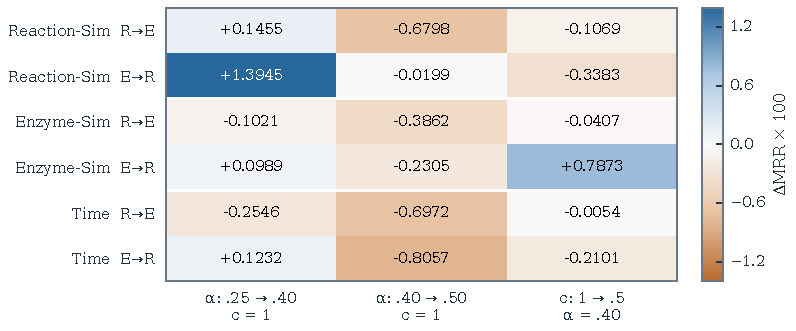
\includegraphics[width=\linewidth]{figures/inference.pdf}
\caption{Inference sensitivity on ReactZyme. Entries are changes in MRR
multiplied by 100 at fixed checkpoints. Each column changes one coefficient;
the common color scale is linear, with blue/orange denoting positive/negative
changes. Rows retain both directions for every split.}
\label{fig:exp-inference}
\end{figure}

\paragraph{Contrastive temperature.}
An 18-epoch EnzymeMap study compares inverse temperatures $\beta=5$ and
$\beta=10$ with paired seeds 17, 42, and 73 and the remaining recipe fixed
(Figure~\ref{fig:exp-temperature}). Lower inverse temperature improves
BEDROC$_{85}$, BEDROC$_{20}$, and EF5 for every seed in both libraries;
seed 73 accounts for the two negative EF10 differences. Mean full-library
BEDROC$_{85}$ increases from $0.4940\pm0.0350$ to $0.5217\pm0.0375$,
where dispersion is sample standard deviation across three seeds. This
supports a temperature effect within the tested objective, but does not
isolate anchor balancing against MLNCE or replicate the final 10-epoch V4
recipe. The 24 metric comparisons are correlated.

\begin{figure}[t]
\centering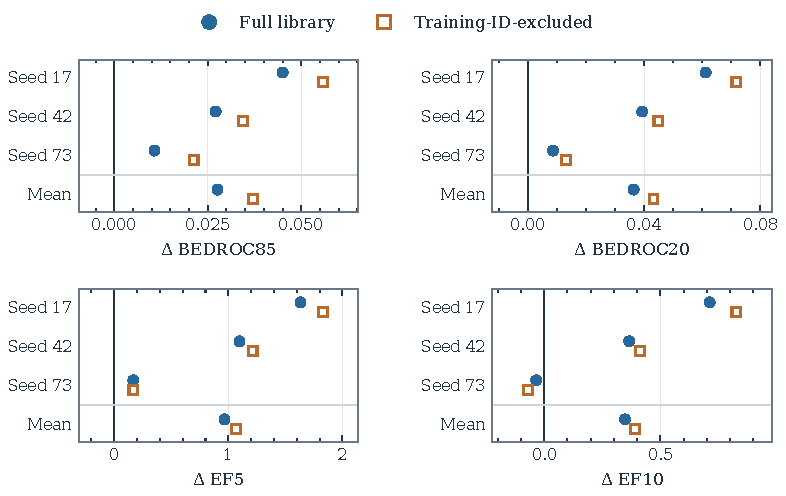
\includegraphics[width=\linewidth]{figures/temperature.pdf}
\caption{Paired temperature effects on EnzymeMap: $\beta=5$ minus
$\beta=10$ at 18 epochs. Circles show the full library and open squares
the training-ID-excluded library. Every seed and their arithmetic mean are
shown. BEDROC differences are unscaled; each metric has its own horizontal
axis. Mean markers do not represent confidence intervals.}
\label{fig:exp-temperature}
\end{figure}

\paragraph{Biological-supervision ablation.}
We augment the proposed phase-2 objective with relative EC, cofactor, and
bond-change losses, with coefficients $(1,1,1)$, margin 0.1, and a fixed
divisor of three. This ablation, denoted \vfourBio, adds no model parameters.
We hold F3 and inference fixed and compare correct phase-2 labels with
shuffled labels and removal of EC, cofactor, or transformation supervision.
Removing a family preserves the other coefficients and divisor of three,
therefore also reducing total regularization. The effects are mixed
(Figure~\ref{fig:exp-biology}). Full-library BEDROC$_{85}$ is 0.572337
without added supervision, 0.572096 with correct labels, and 0.572093 with
shuffled labels. All five controls slightly reduce both BEDROC endpoints
in both libraries. On ReactZyme, the larger Enzyme-Sim/Time E$\to$R changes
are sensitive to near-equal scores: optimistic and pessimistic rankings
within a $10^{-6}$ score band overlap substantially between V4 and V4+Bio.
The Time increase from 0.7807 to 0.8006 therefore does not alone establish
robustly improved discrimination. These bounds measure numerical sensitivity,
not sampling uncertainty.

\begin{figure}[t]
\centering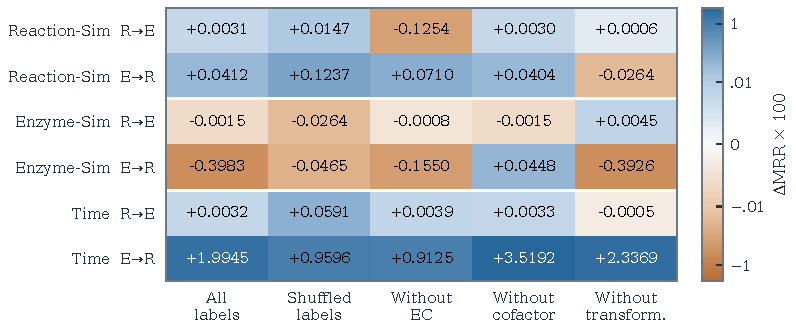
\includegraphics[width=\linewidth]{figures/biology.pdf}
\caption{Phase-2 biological supervision on ReactZyme. Values are
$100\Delta\mathrm{MRR}$ relative to V4. Colors share a symmetric logarithmic
scale, linear within $\pm0.001$ displayed units; printed values are
untransformed. Small effects remain visible without independent row scaling.
The largest E$\to$R changes require the near-tie qualification in the text.}
\label{fig:exp-biology}
\end{figure}

A separate study applies biology during F3 training with paired seeds
42, 43, and 44 and leaves phase 2 unannotated. Weight 1 increases mean
full-library BEDROC$_{85}$ by 0.0103 but lowers mean EF5 by 0.1514; only
two of three seeds improve BEDROC$_{85}$. EF5 decreases in the excluded
library for all three seeds. Weight 0.1 improves excluded-library EF10 for
all seeds, but not every other endpoint. Both training stages therefore
show metric-dependent biological-loss effects. The available sensitivities
do not replace matched removals of the dictionary, phase 2, or learned
residue views.

\subsection{Case1: recovery of literature-supported tagatose catalysts}
\label{sec:exp-case1}

\paragraph{Reaction and candidate panel.}
Case1 concerns direct C4 epimerization of free D-fructose to D-tagatose.
We assemble a targeted panel from the literature, including engineered
UxaE variants and characterized tagatose 4-epimerases
\citep{caseS01,caseS02,caseS03,caseS04,caseS05,caseS06,caseS16,caseS17}.
The catalogue contains 145 entries; one construct, H017 (KoT4E M6), lacks
a fully recoverable sequence. We therefore rank 144 resolved entries,
representing 123 unique sequences. The primary-paper evidence set contains
12 unique sequences or 15 entries. Broader workbook annotations identify
81 active sequences and 42 with conditional non-detection evidence; these
heterogeneous labels are used only for a secondary conditional AUROC.
The curated candidate ranking is not treated as an activity label.

\paragraph{Evaluation.}
We use the Reaction-Sim-trained model as the primary deployment without
fitting its retrieval parameters to Case1 labels. Recovery is measured
against primary-paper positives in both candidate views. Uniform random
ranking would recover an expected $25(12/123)=2.44$ unique positives or
$25(15/144)=2.60$ positive entries at rank 25. These expectations are
descriptive references, not confidence intervals. The case was examined
during development and is a retrospective literature evaluation, rather
than an untouched prospective wet-lab experiment.

\begin{table}[t]
\centering\small
\caption{Case1 primary-paper recovery at rank 25. Unique recovery is out
of 12 positives among 123 sequences; entry recovery is out of 15 among 144
resolved entries. AUROC uses the broader 81/42 conditional workbook labels.
The EnzymeMap model is a transfer diagnostic.}
\label{tab:exp-case1}
% Generated from bundled frozen evidence; stages uses stage_comparison.json.
\begingroup\setlength{\tabcolsep}{2.8pt}
\begin{tabular}{@{}lrrr@{}}
\toprule
Model & Unique @25 & Entries @25 & AUROC \\
\midrule
Native F3 & 9/12 & 10/15 & 0.6008 \\
\methodname & 10/12 & 10/15 & 0.6129 \\
V4 (EnzymeMap) & 6/12 & 6/15 & 0.4706 \\
\bottomrule
\end{tabular}
\endgroup

\end{table}

\paragraph{Results.}
\methodname\ recovers 10/12 unique paper-supported catalysts at rank 25,
compared with 9/12 for its native F3 encoder before phase 2
(Table~\ref{tab:exp-case1}), and recovers 10/15 positives in the 144-entry view.
The biological-supervision ablation recovers 11/12 unique catalysts while
retaining 10/15 entry-level recovery. The additional unique hit
is TsT4Ease WT, which moves from rank 26 to 25. Cofactor removal retains
this gain, whereas label shuffling and transformation removal do not
(Figure~\ref{fig:exp-case1}). Conditional AUROC changes only from 0.6129
to 0.6138. V4 retrieves no primary-paper catalyst among its first five
unique sequences and three among its first ten, showing that top-25
recovery does not imply strong very-early prioritization.

\begin{figure}[t]
\centering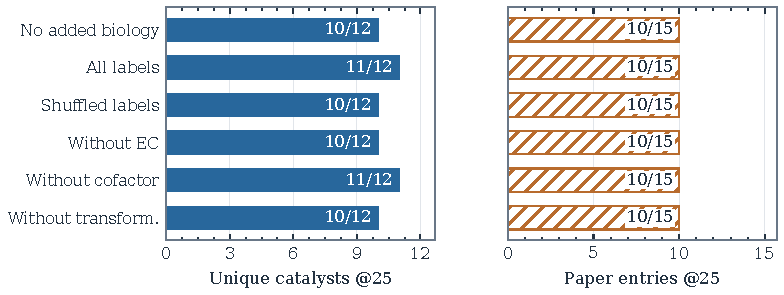
\includegraphics[width=\linewidth]{figures/case1.pdf}
\caption{Case1 phase-2 controls using the same Reaction-Sim model lineage.
Left: unique-sequence recovery at 25; right: original-entry recovery at 25.
Blue filled and orange hatched bars distinguish the evaluation units, with
their positive denominators printed explicitly. The one-sequence gain
does not increase entry-level recovery.}
\label{fig:exp-case1}
\end{figure}

The EnzymeMap-trained model recovers 6/12 unique positives and has
conditional AUROC 0.4706, indicating weaker transfer despite its strong
screening benchmark performance. Furthermore, four of the ten positives
recovered by Reaction-Sim V4 have identified training homologs with at
least 90\% identity, and both query molecules co-occur in larger training
participant sets. Frozen-backbone exposure is not ruled out. Case1 thus
supports prioritization within this targeted panel, with limited evidence
for distant catalytic generalization.

\paragraph{Scope of the evidence.}
The experiments establish improved EnzymeMap early retrieval under two
released screening protocols, competitive published-reference ReactZyme
scores, and retrospective recovery of documented catalysts. They also
identify a stronger matched-data ReactZyme comparator and mixed effects
from added biology. The final recipe followed repeated exploratory test
inspection; primary results are single-seed estimates. Replication of the
final recipe and evaluation on a prospectively specified external reaction
panel are needed to establish broader generalization.
